
\documentclass{standalone}

%\documentclass[convert]{standalone}
% convert: in addition to pdf output files, png files are created
% convert options does work properly with -output-directory option of latexmk

\usepackage{tikz-feynman}
\tikzfeynmanset{compat=1.1.0}

\usepackage{ulem}
\newcommand{\MET}{\not\hspace{-0.14cm}E_T}

\begin{document}
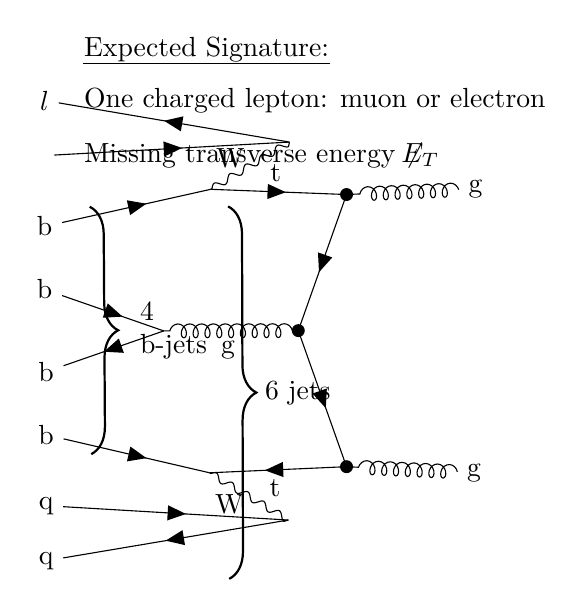
\begin{tikzpicture}
      \begin{feynman}
        \diagram [vertical=a to c] {
            % ttbb production, t-channel, copy from theory
            gi1 [particle=g]
            -- [gluon] a [dot],
            qf1 -- [fermion, edge label=t] a,
            a -- [fermion] b [dot],
            b -- [gluon, edge label=g] addgluon,
            b --  [fermion] c [dot],
            gi2 [particle=g]
            -- [gluon] c
            --  [fermion, edge label=t] qf2,

            b1 [particle=b] -- [fermion] addgluon -- [fermion] b2 [particle=b],

            % invisible helper lines for layout
            gi1 -- [draw=none] ih1 -- [draw=none] gi2,
            qf1 -- [draw=none] addgluon -- [draw=none] qf2,
            qf1 -- [draw=none] ih2 -- [draw=none] b1,
            qf2 -- [draw=none] ih3 -- [draw=none] b2,
            b1 -- [draw=none] b2,
            };

            %
            % additional nodes, after layouting algorithm done
            %

            % top quark (top of graph)
            %\vertex [above right=of qf1] (w1);                  % relative to top quark
            \vertex [right= 1cm of qf1] (t1_invis_helper);    % helper
            \vertex [above=0.6cm of t1_invis_helper] (w1);
            \draw [boson] (qf1) -- (w1) node[near start, above] {W};
            % \vertex [below right=of qf1] (t1b) {b};            % relative to top quark
            \vertex [above=0.8cm of b1] (t1b) {b};             % relative to b1 from bb pair
            % \vertex [below=0.6cm of t1_invis_helper] (t1b) {b};  % relative to helper
            \draw [fermion] (t1b) -- (qf1);

            % neutrino
            \vertex [above=1.7cm of b1] (t1nu) {\nu};             % relative to b1 from bb pair
            \draw [fermion] (t1nu) -- (w1);

            % charged lepton
            \vertex [above=2.4cm of b1] (t1l) {$l$};             % relative to b1 from bb pair
            \draw [fermion] (w1) -- (t1l);


            % top quark (bottom of graph)
            \vertex [right= 1cm of qf2] (t2_invis_helper);    % helper
            \vertex [below=0.6cm of t2_invis_helper] (w2);
            \draw [boson] (qf2) -- (w2) node[near start, below] {W};
            \vertex [below=0.8cm of b2] (t2b) {b};             % relative to b1 from bb pair
            \draw [fermion] (t2b) -- (qf2);

            % W->q1
            \vertex [below=1.7cm of b2] (t2nu) {q};             % relative to b1 from bb pair
            \draw [fermion] (t2nu) -- (w2);

            % W->q2
            \vertex [below=2.4cm of b2] (t2l) {q};             % relative to b1 from bb pair
            \draw [fermion] (w2) -- (t2l);

            % b jets brace
            \draw [decoration={brace, amplitude=10pt, raise=10pt}, decorate, thick] (t1b.north east) -- (t2b.south east)
                node [midway, xshift=40pt, align=left] (bjets_brace) {4\\b-jets};

            % all jets brace
            \draw [decoration={brace, amplitude=10pt, raise=60pt}, decorate, thick] (t1b.north east) -- (t2l.south east)
                node [midway, xshift=85pt] {6 jets};

            % charged lepton label
            % \draw[anchor=west]  let \p{A}=(b1.east), \p{B}=(t1l) in (\x{A} + 5pt, \y{B}) node (lepton_label) {One charged lepton: muon or electron};
            % \draw[anchor=west]  let \p{A}=(b1.east), \p{B}=(t1nu) in (\x{A} + 5pt, \y{B}) node {Missing transverse energy $\MET$};

            % -20 pt x offset =
            \draw[anchor=west]  let \p{A}=(bjets_brace.west), \p{B}=(t1l) in (\x{A} - 20pt, \y{B}) node (lepton_label) {One charged lepton: muon or electron};
            \draw[anchor=west]  let \p{A}=(bjets_brace.west), \p{B}=(t1nu) in (\x{A} - 20pt, \y{B}) node {Missing transverse energy $\MET$};

            %\node[draw=none, anchor=west] [above= 0.8 cm of lepton_label] {\uline{Expected Signature:}};
            \draw[anchor=west]  let \p{A}=(lepton_label.west) in (\x{A}, \y{A} + 18pt) node {\uline{Expected Signature:}};


      \end{feynman}
    \end{tikzpicture}
\end{document}
